\section{Projected Results}

To perform the simulation study and obtain the projected results, we developed
a DEMP generator, as discussed in Appendix-A, and used it to generate events
within a kinematic phase space slightly larger than the SoLID-SIDIS acceptance.
The Fermi motion of the neutron in $\mathrm{^{3}He}$ and the radiative effects have
been taken in account in this generator.  Then for every detected
particle in each event, we added the acceptance profiles obtained from the
GEANT4 simulation with the SoLID-SIDIS configuration.

\subsection{Kinematic Coverage}
\begin{figure}[!ht]
 \begin{center}
      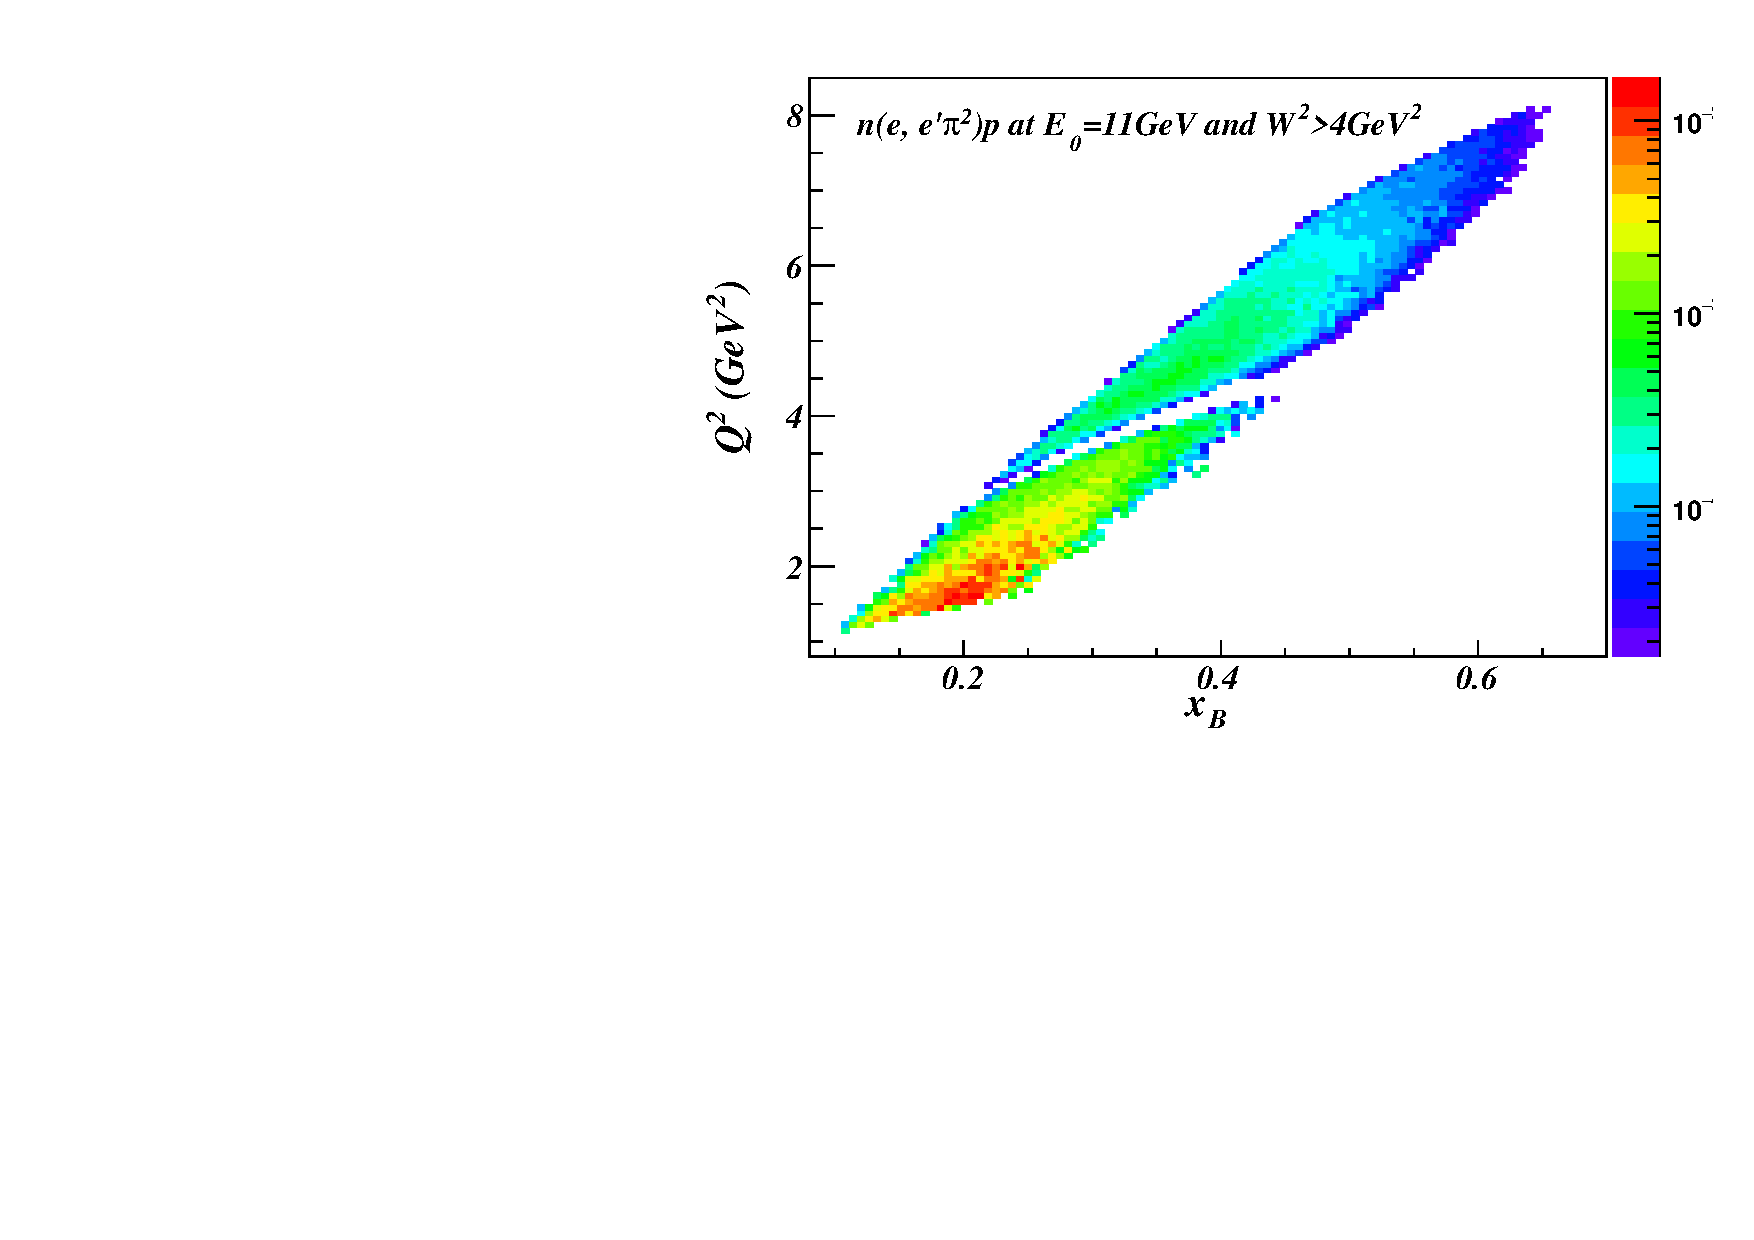
\includegraphics[type=pdf,
        ext=.pdf,read=.pdf,width=0.45\textwidth]{./figures//Q2_x_02Hz}
  
   \caption{\footnotesize{The
kinematic coverage at 11~GeV within the SoLID acceptance. A cut $W^2>$4~GeV$^2$ was applied. }}
  \label{kin_cor}
  \end{center}
\end{figure}
The kinematic coverage in $Q^{2}$ vs. $x_{B}$ is shown in Fig.~\ref{kin_cor},
using the existing SoLID detectors to detect electrons, pions and protons at
$8^{\circ}\sim24^{\circ}$. These distributions were
weighted by the DEMP unpolarized cross sections and the SoLID acceptance profiles for electrons, pions and protons. 
A cut $W^{2}>4~GeV^{2}$ was also applied to exclude non-DIS events.
\begin{figure}[!ht]
 \begin{center}
   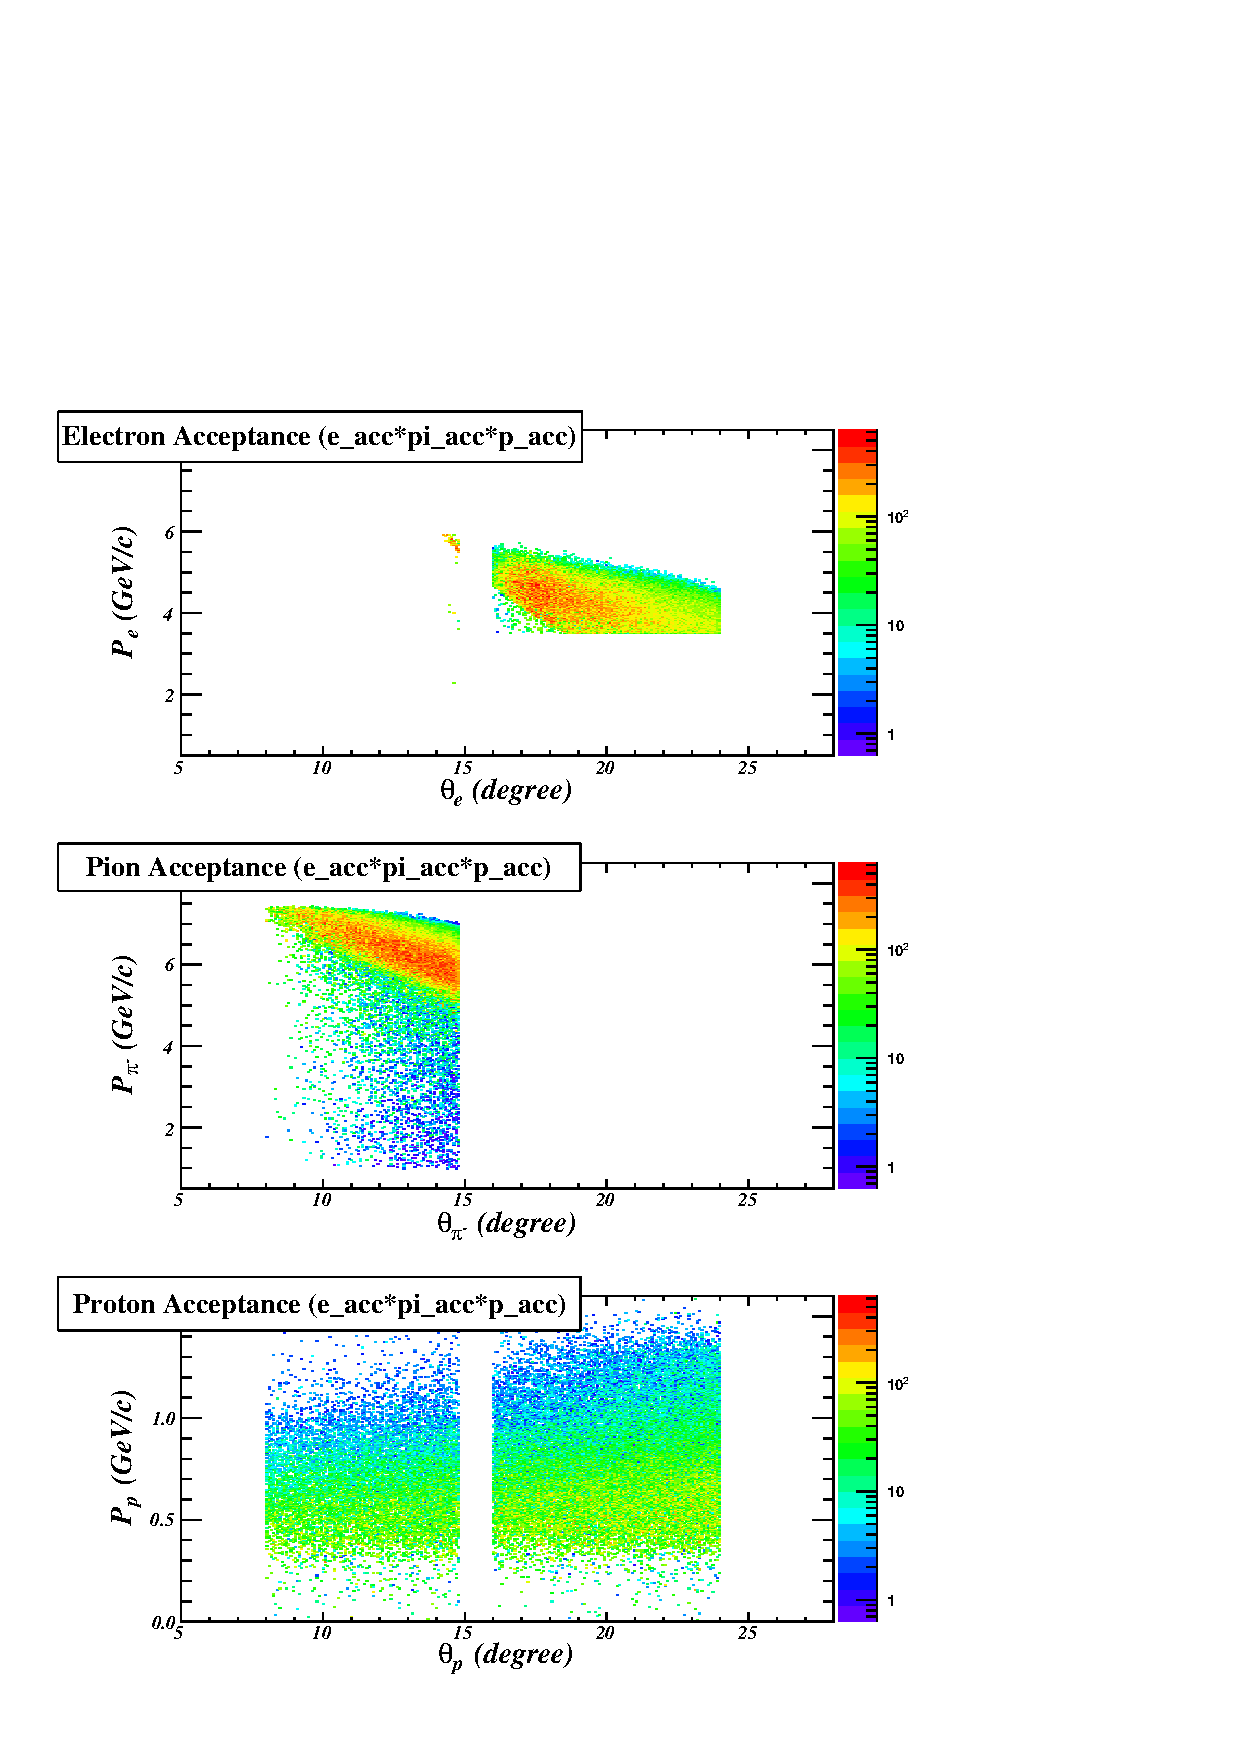
\includegraphics[type=pdf,
     ext=.pdf,read=.pdf,width=0.45\textwidth]{./figures/E11_acc_epip_Q2gt4_02Hz}
   \caption[The acceptance of the momenta and scattering angles for electrons,
    $\pi^{-}$ and protons]{\footnotesize{The acceptance of the momenta and
polar angles. The top, middle and bottom plots are for electrons, $\pi^{-}$ and
protons, respectively. Cuts of $Q^{2}>4~\mathrm{GeV^{2}}$ and $W^2>$4~GeV$^2$ were applied.}}
  \label{p_theta}
  \end{center}
\end{figure}

Fig.~\ref{p_theta} shows the momentum and angular acceptance of electrons,
$\pi^{-}$ and protons which form the DEMP events and can be detected with the
SoLID detectors.  Cuts of $Q^{2}>4~\mathrm{GeV^{2}}$ and $W^2>$4~GeV$^2$ were applied since this is the region
of greatest physics interest.  The recoil protons shown in Fig.~\ref{p_theta} have low momenta ranging from 0.3~GeV/c up
to 1.2~GeV/c and their rates are distributed nearly uniformly in scattering
angle.

\subsection{Estimated Rates
\label{sec:rates}}

\begin{table}[!ht]
\centering
\begin{tabular}{|c|c|}
 \hline
  $Q^2>$1~GeV$^2$ & $Q^2>$4~GeV$^2$\\
 \hline
\multicolumn{2}{|c|}{DEMP: $\vec{n}(e,e'\pi^{-}p)$ Triple-Coincidence (Hz)}\\
 \hline
 4.22   &  0.20 \\
 \hline
\multicolumn{2}{|c|}{SIDIS: $\vec{n}(e,e'\pi^{-})X$ Double-Coincidence (Hz)}\\
 \hline
   1424.62  & 35.77   \\
 \hline
\end{tabular}
\caption[Triple-Coincidence rates for
  neutron-DEMP]{\footnotesize{Triple-Coincidence rates for DEMP events compared
    with the SIDIS rates. A cut $W^2>$4~GeV$^2$ was applied. The online production
    trigger will be the SIDIS double-coincidence trigger of which rates are
    also given.}}
\label{rate_table}
\end{table} 

Table~\ref{rate_table} lists the triple-coincidence rate of the DEMP
events after applying cuts on . The rates were calculated with the simulated events weighted by the
target luminosity, the SoLID acceptances and unpolarized cross sections.  The
``raw'' rates are not corrected by the beam and target polarization, target
dilution and so on.  Our conservatively estimated rate is around 4.22~Hz at $Q^{2}>$1~GeV$^{2}$, or 0.20 Hz
at $Q^{2}>$4~GeV$^{2}$. For comparison, the table also gives the SIDIS rate
which will be the online production trigger rates and is the main background of
the DEMP events.

\subsection{Asymmetry Projections}
\begin{figure}[!ht]
 \begin{center}
      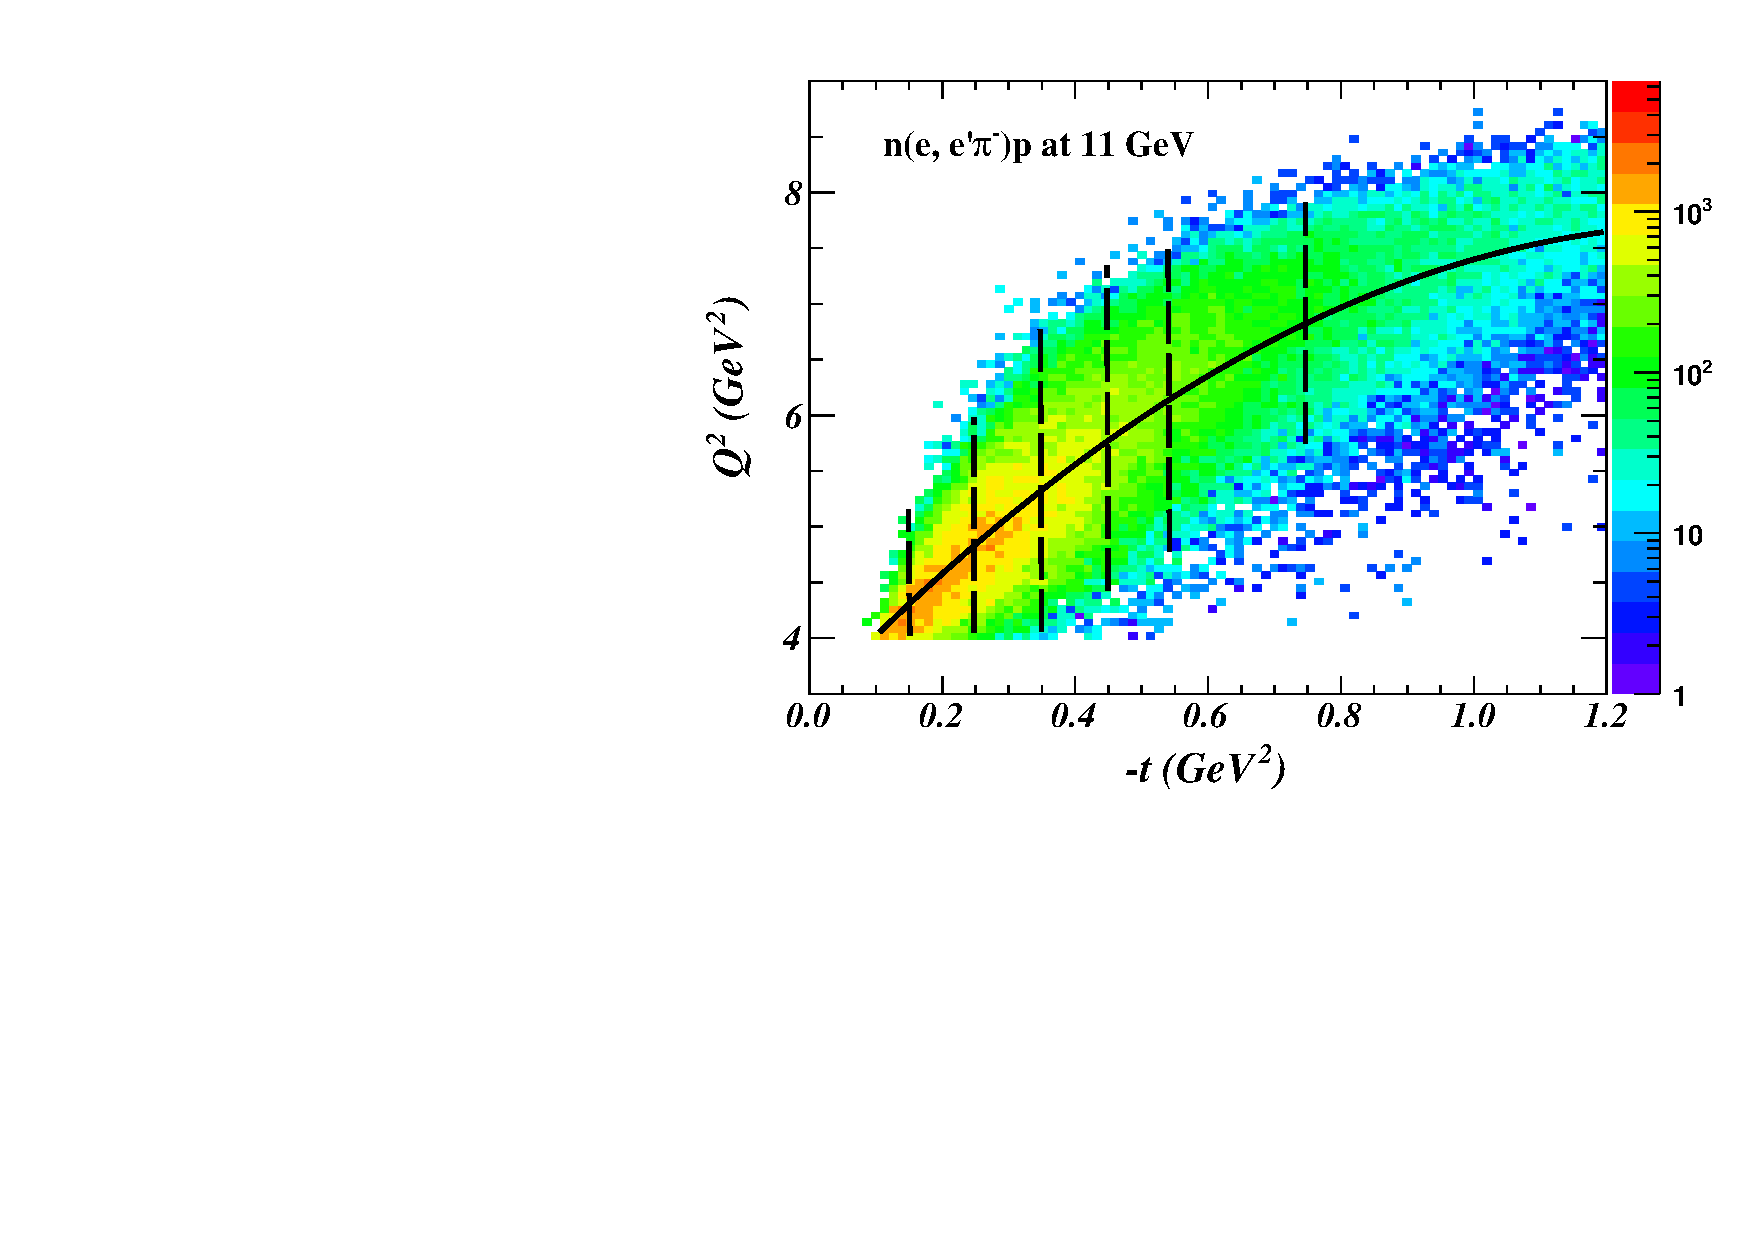
\includegraphics[type=pdf,
        ext=.pdf,read=.pdf,width=0.5\textwidth]{./figures/E11_Q2_t_bin_02Hz} 
    \caption[$Q^{2}$ vs. $-t$]{\footnotesize{$Q^{2}$ vs. $-t$ where the black
dashed lines specify the boundaries of 7 $-t$ bins and the black dash-dot lines
indicate the additional two $Q^{2}$ bins. }}
  \label{Q2_t_bin}
  \end{center}
\end{figure}

The proposed experiment will run in parallel with E12-10-006, which has already
been approved to run 48 days at $E_{0}$=11~GeV.  As shown in
Fig.~\ref{Q2_t_bin}, we defined 7 $-t$ bins of which the boundaries are
defined by the array:
 \begin{equation}
-t[8] = [0.0, 0.15, 0.25, 0.35, 0.45, 0.55, 0.75, 1.10]~~~~(\mathrm{in~GeV^{2}})
 \end{equation}
The number of events ($N_{i}$) in the $i$th bin is calculated from the total
simulated events after applying cuts on important kinematic variables,
e.g. $Q^{2}>$4~GeV$^{2}$, $W>$2~GeV, 0.55$<\epsilon<$0.75 and
$-t_{min}<-t<-t_{max}$. As shown in Eqn.~\ref{ncount}, each event surviving the
cuts is then weighted by the unpolarized cross section, together with the
acceptance of the electron, pion and proton. $N_{i}$ is further corrected by
the phase-space factor ($PSF$) defined in the event generator, the total number
of randomly generated events ($N_{gen}$), beam-time ($T$), the target
luminosity ($L=10^{36}$~cm$^{-2}$s$^{-1}$), and the overall detector efficiency 
($\epsilon_{eff}$):
 \begin{equation}
     N_{i} = \bigl(\sum_{j\in i-bin} \sigma_{j}\cdot A^{e}_{j} \cdot
     A^{\pi^{-}}_{j} \cdot A^{p}_{j}\bigr) \cdot (PSF/N_{gen}) \cdot T \cdot L \cdot
     \epsilon_{eff},
     \label{ncount}
 \end{equation}
where $j$ is the $j$th event in the $i$th bin, $\sigma_{j}$ is the cross
section of the $j$th event. $A^{e(\pi^{-},p)}_{j}$ is the acceptance weight of the
electron (pion, proton) in this event. The detector efficiency,
$\epsilon_{eff}$, is approximately fixed at 85\% as was used in SIDIS
proposals. $N_{i}$ corresponds to the raw experimental count of electrons
scattering on neutrons in $\mathrm{^{3}He}$ before taking into account the
target polarization ($P\sim60\%$), the effective polarization of neutrons
($\eta_{n}\sim0.865$), and the dilution effect from other reaction channels
when electrons scattering on $\mathrm{^{3}He}$ ($f \sim 0.9$). 

In addition, we further divide each $-t$-bin into two $Q^{2}$ bins with similar
statistics.  By doing that, we are able to examine the $Q^{2}$-dependence of the
asymmetries, and also check the model dependence of the other corrections that
are directly related to the values of $Q^{2}$.

The statistical error of the target single spin asymmetry ($A_{UT}$) in each
bin can be given as:
  \begin{equation}
    \delta A_{UT} = \frac{1}{P\cdot\eta_{n}\cdot f} \sqrt{\frac{1-(P\cdot
        <A_{UT}>)^{2}}{N^{+}_{i}+N^{-}_{i}}},
    \label{stat_err}
 \end{equation}
where $N^{+(-)}_{i}$ is the number of counts in each bin when the target
polarization is up (down), and we easily have $N_{i}=N^{+}_{i}+N^{-}_{i}$;
$<A_{UT}>$ is the average asymmetry in the bin, and experimentally, it can be
extracted as the following:
\begin{equation}
   <A_{UT}> = \frac{1}{P\cdot\eta_{n}\cdot f} \frac{N^{+}-N^{-}}{N^{+}+N^{-}}.
   \label{asym_exp}
\end{equation}
In this projection study, $A_{UT}$ is predicted with a phenomenological model,
as discussed in Appendix-A. Because of not performing a L/T separation in this
experiment, the asymmetry should be corrected by another dilution factor, which
is defined as:
\begin{equation}
  f_{L/T} =\frac{\epsilon\sigma_{L} }{\sigma_{T}+\epsilon\cdot\sigma_{L} },
\end{equation} 
where $\epsilon=(1+\frac{2\nu^{2}}{Q^{2}}\tan^{2}(\theta))^{-1}$. Additional
dilution due to $\sigma_{TT}$ is assumed to be small.  A factor of $-1$ is also
applied after comparing Eq.~\ref{eqn:asy} and Eq.~\ref{eqn:sigtarg}. Hence,
$A_{UT} = -f_{L/T}\cdot A_{L}^{\perp,model}$.

\begin{figure}[!ht]
 \begin{center}
               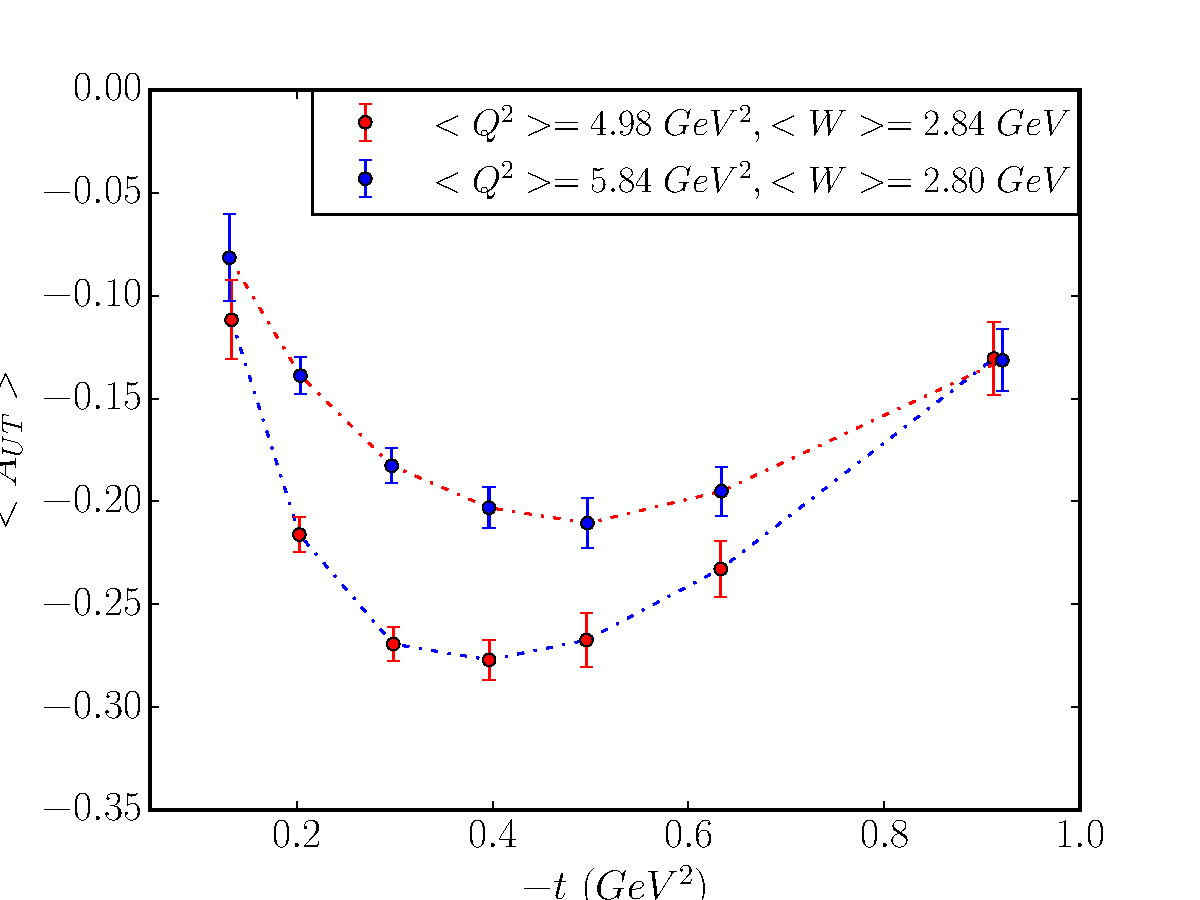
\includegraphics[type=pdf,
        ext=.pdf,read=.pdf,width=0.65\textwidth]{./figures/bin_asym_t_fermi_02Hz} 
      
      \caption{\footnotesize{Projection of target single spin asymmetry
          ($A_{UT}$) as a function of $-t$ for DEMP with transversely polarized
$\mathrm{^{3}He}$ at $E_{0}$=11~GeV (directly compare with
Fig.~\ref{fig:hermes_aut}).  The data in each $-t$ bin are further divided into
two $Q^{2}$ bins with similar statistics.  The error bars include only the
projected statistical uncertainties defined in Eq.~\ref{stat_err}. The
asymmetry value in each bin is predicted with the model given in Appendix-A and
is diluted due to not separating the L/T contributions.}}
  \label{asym_t}
  \end{center}
\end{figure}

Fig.~\ref{asym_t} shows the distribution of $A_{UT}$ vs. $-t$ with projected
statistical errors discussed above. Compared with the existing HERMES results
(Fig.~\ref{fig:hermes_aut}), the new measurement could provide more precision
data to be directly compared with theoretical predictions. Extra binning on
$Q^{2}$ enables us to study the $Q^{2}$-dependence of asymmetries as well as to
constraint some corrections during the asymmetry extraction.  The detailed
information of each bin is listed in Table~\ref{asym_bin_table}.  
\begin{table}[!ht]
\centering
 \small
\begin{tabular}{|c|c|c|c|c|c|c|c|}
\hline
 \multicolumn{8}{|c|}{$Q^{2}$ bin-set\#1 } \\
\hline
      &  t-bin\#1 & t-bin\#2 & t-bin\#3 & t-bin\#4 & t-bin\#5 & t-bin\#6 & t-bin\#7 \\
  \hline
$<-t>$    &  0.13 &  0.20 & 0.30 & 0.40 & 0.50 & 0.63 & 0.91 \\
$<Q^{2}>$   &  4.11 &  4.36 & 4.73 & 5.10 & 5.48 & 5.96 & 6.66 \\
$<\sigma_{L}/\sigma_{T}>$    &  6.31 &  4.84 & 3.55 & 2.73 & 2.14 & 1.48 & 0.58 \\
$<f_{L/T}>$   &  0.80 &  0.76 & 0.70 & 0.64 & 0.58 & 0.48 & 0.26 \\
$<A_{UT}>$ &  -1.12$\times 10^{-1}$ &  -2.16$\times 10^{-1}$ & -2.69$\times 10^{-1}$ & -2.77$\times 10^{-1}$ & -2.67$\times 10^{-1}$ & -2.33$\times 10^{-1}$ & -1.31$\times 10^{-1}$ \\
$\delta A_{UT}$  &  1.92$\times 10^{-2}$ &  8.49$\times 10^{-3}$ & 8.18$\times 10^{-3}$ & 9.64$\times 10^{-3}$ & 1.32$\times 10^{-2}$ & 1.37$\times 10^{-2}$ & 1.76$\times 10^{-2}$ \\
\hline

\multicolumn{8}{|c|}{$Q^{2}$ bin-set\#2 } \\
\hline
      &  t-bin\#1 & t-bin\#2 & t-bin\#3 & t-bin\#4 & t-bin\#5 & t-bin\#6 & t-bin\#7 \\
  \hline
$<-t>$     &  0.13 &  0.20 & 0.30 & 0.40 & 0.50 & 0.63 & 0.92 \\
$<Q^{2}>$   &  4.35 &  4.87 & 5.45 & 5.98 & 6.43 & 6.92 & 7.63 \\
$<\sigma_{L}/\sigma_{T}>$   &  7.05 &  6.08 & 5.13 & 4.27 & 3.37 & 2.31 & 0.96 \\
$<f_{L/T}>$     &  0.81 &  0.79 & 0.76 & 0.73 & 0.68 & 0.59 & 0.36 \\
$<A_{UT}>$   &  -8.15$\times 10^{-2}$ &  -1.39$\times 10^{-1}$ & -1.83$\times 10^{-1}$ & -2.03$\times 10^{-1}$ & -2.11$\times 10^{-1}$ & -1.95$\times 10^{-1}$ & -1.31$\times 10^{-1}$ \\
$\delta A_{UT}$   &  2.20$\times 10^{-2}$ &  9.17$\times 10^{-3}$ & 8.91$\times 10^{-3}$ & 1.04$\times 10^{-2}$ & 1.25$\times 10^{-2}$ & 1.23$\times 10^{-2}$ & 1.57$\times 10^{-2}$ \\
\hline
\end{tabular}
\caption[Detailed information of projected bins]{\footnotesize{Detailed
information of projected bins from the new DEMP measurements with SoLID, while
$<Q^{2}>$ and $<-t>$ are in the unit of GeV$^{2}$. The data are
divided into 14 $-t$ bins in both $-t$ (7 bins) and $Q^{2}$ (2 bins).  The
projected uncertainties are statistical only.}}
\label{asym_bin_table}
\end{table} 

\subsection{Missing Mass and Background}

In the DEMP reaction on a neutron, all three charged particles in the final
state, $e^{-}$, $\pi^{-}$ and $p$, can be cleanly measured by the SoLID detector
system.  Hence, contamination from other reactions, including
DEMP with other two protons in $^{3}He$, can be greatly eliminated.  The
dominant background of the DEMP measurement comes from the SIDIS reactions of
electrons scattering on the neutron and two protons in $\mathrm{^{3}He}$. In
addition to detecting the recoil protons, which should largely suppress most of
background, we will also rely on reconstructing the neutron missing mass
spectrum to ensure the exclusivity of the DEMP events. In SIDIS, however, the
final states include the scattered electron, the hadrons ($\pi^{\pm}$,
$K^{\pm}$ etc.), as well as the undetected target fragments which could contain
protons. Hence, the SIDIS events will possibly leak into the DEMP missing mass
spectrum.

We studied the contamination of the SIDIS events in the DEMP missing momentum
and mass spectra. The SIDIS reactions, $p(e,e'\pi^{-})X$ and $n(e,e'\pi^{-})X$,
were simulated with the same generator used for the SoLID-SIDIS proposals, and
their rates were calculated by matching the acceptance of scattered electrons
and pions with the ones in DEMP. We then fold the SoLID detector resolutions
into the spectra. Based on the current tracking study, the SoLID-SIDIS system
can provide a momentum resolution of $2\%/\sqrt{E}$, a polar angle
resolution of 0.6~mrad, an azimuthal angle resolution of 5~mrad and a
vertex target position of 0.5~cm. It is difficult to estimate what
percentage of the SIDIS target fragments contain protons, so we assumed
the target fragments ($``X''$) all contain one or more protons. Such an
assumption likely results in the SIDIS background being significantly
overestimated.

\begin{figure}[!ht]
\begin{center}
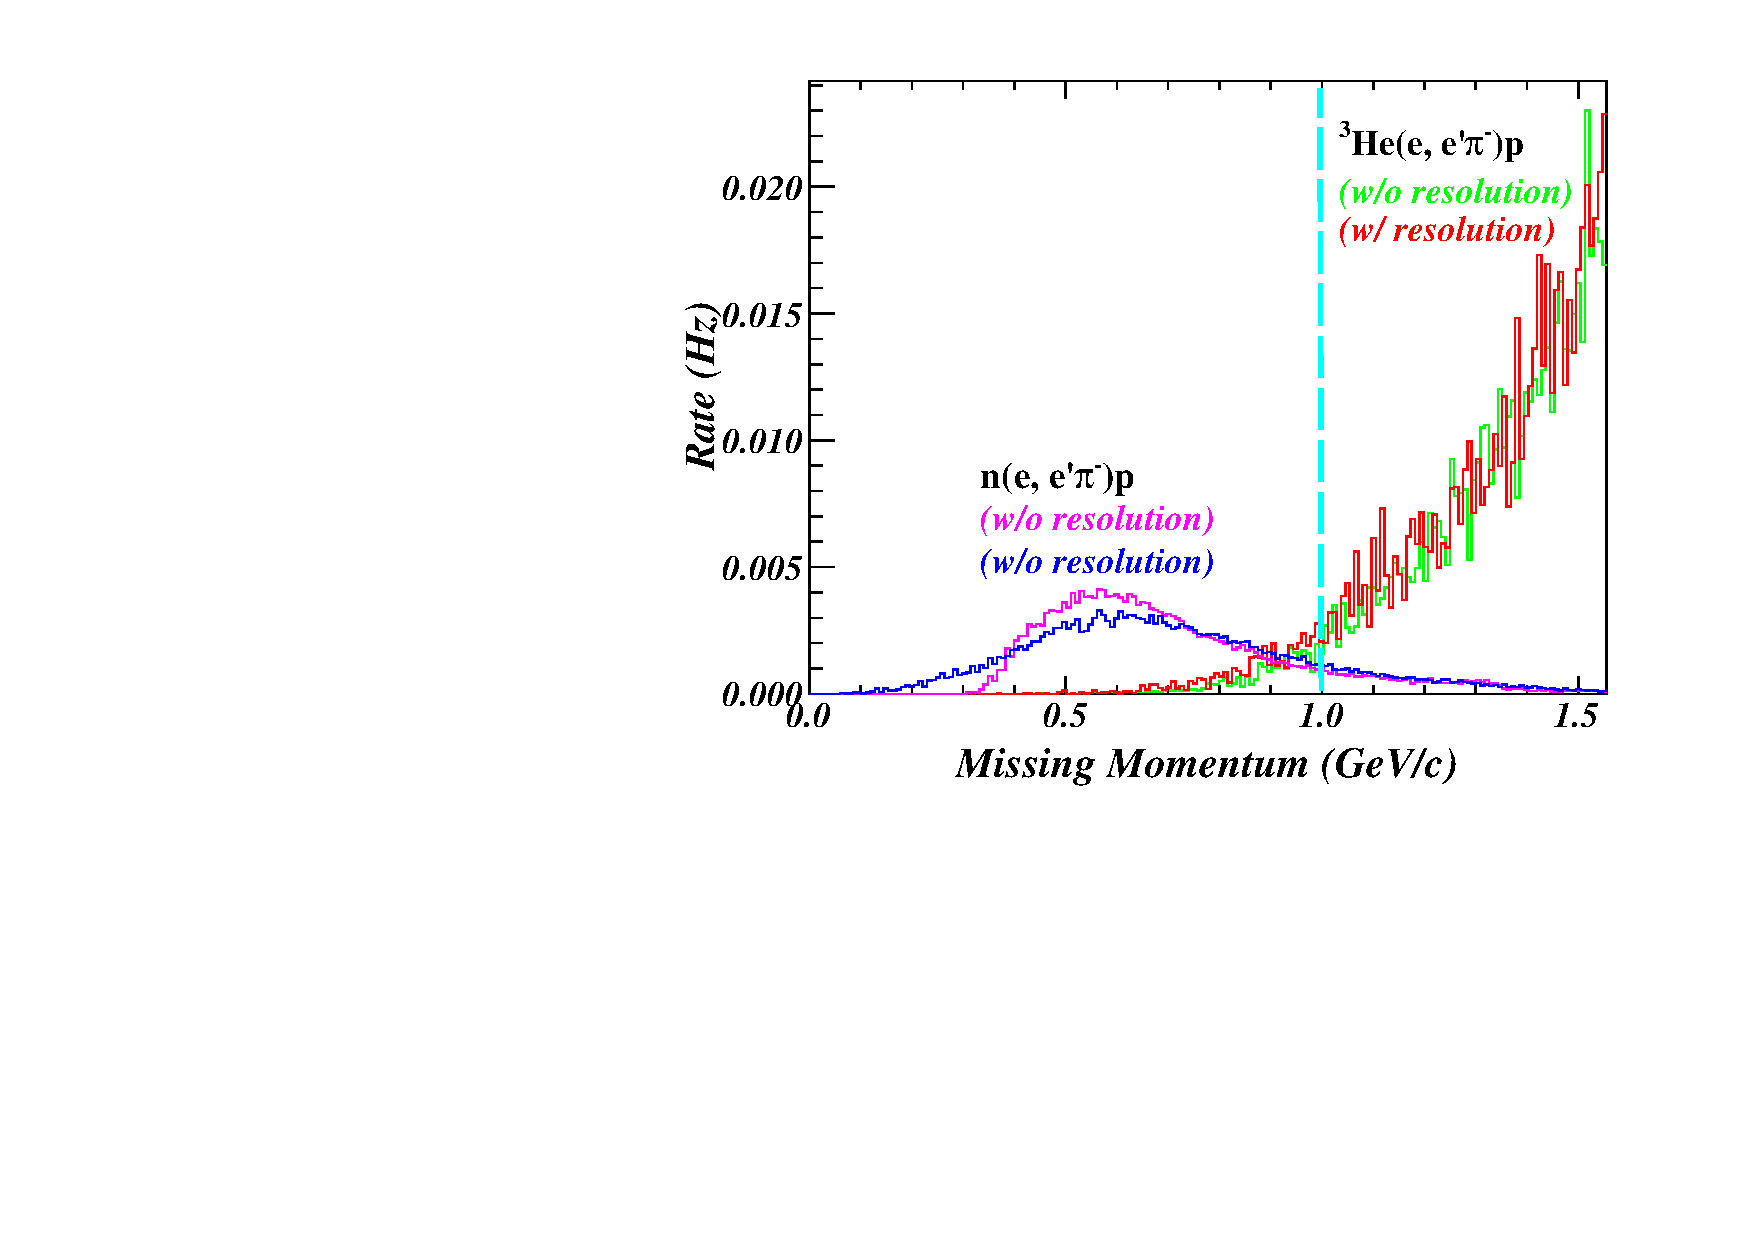
\includegraphics[type=pdf,ext=.pdf,read=.pdf,width=0.5\textwidth]
{./figures/Missing_P_Fermi_Rad_02Hz}
\caption[Missing Momentum]{\footnotesize{Missing momentum spectra of DEMP and
SIDIS events in the worse scenario where we assume all SIDIS events contain protons in the final state. 
The missing momentum distributions are well separated between the
two processes and one can apply a cut at $P_{miss}<1.0$~GeV/c (indicated by the
light-blue dashed line) to remove most of the SIDIS events. }}
  \label{missing_mom}
  \end{center}
\end{figure}

Fig.~\ref{missing_mom} shows a reconstruction of the missing momenta of both
processes. One immediately sees that the missing momentum distributions of two
processes are well separated.  The SIDIS background can be largely rejected
when we apply a cut, $P_{miss}<1.0$~GeV/c. 

\begin{figure}[!ht]
 \begin{center}
      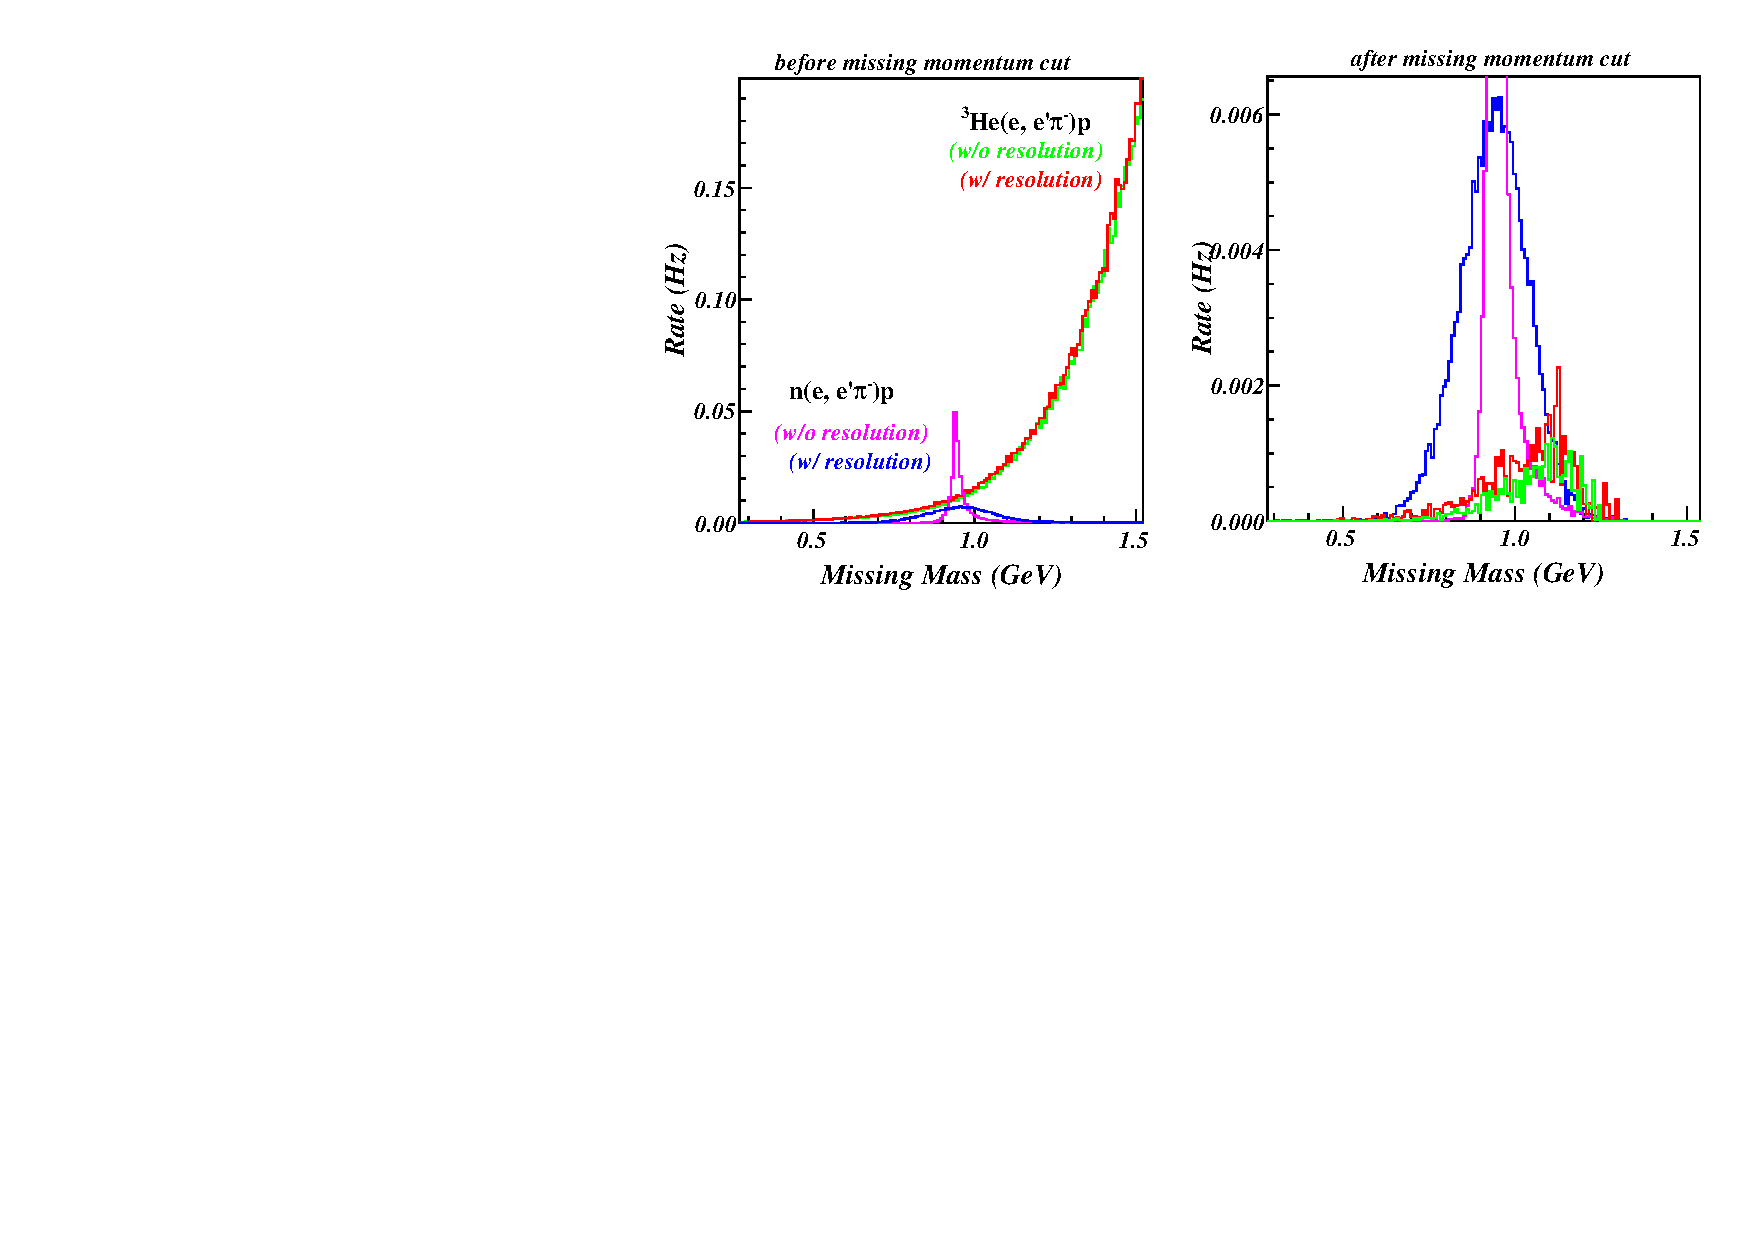
\includegraphics[type=pdf,
        ext=.pdf,read=.pdf,width=0.85\textwidth]
{./figures/Missing_Mass_Fermi_Rad_02Hz} \\
   \caption[Missing Mass]{\footnotesize{Missing mass spectra of DEMP and SIDIS
events in the worse scenario where we assume all SIDIS events contain protons in the final state. 
Top (bottom) panel shows the missing mass distribution of DEMP events.
The left (right) plot of each panel shows the background contamination from
SIDIS events before (after) the missing momentum cut shown in
Fig.~\ref{missing_mom}. The broadening effect of the missing mass due to the
Fermi motion and the energy loss is indicated by the magenta curve. The SIDIS
background is already small compared with DEMP events before optimizing the
cut. The actual SIDIS background should be much smaller, since we overestimated
the SIDIS rate by assuming all target fragments $"X"$') in the SIDIS process
contain protons.}}
  \label{missing_mass}
  \end{center}
\end{figure}

We then reconstructed the missing mass spectra of the DEMP and SIDIS events w/
and w/o the missing momentum cuts, as shown in Fig.~\ref{missing_mass}. Before
applying the missing momentum cut, the SIDIS background overwhelms the DEMP
peak (note that, however, the SIDIS rate is likely overestimated). After
applying the cut, the DEMP peak dominates and the SIDIS background is largely
suppressed. The total integrated SIDIS becomes 0.04Hz compared with the rate of DEMP rate (0.2Hz).
 If we consider the fact that not every $``X''$ in SIDIS contains a
proton, the remaining background should be negligible.

Other random coincident background events will show up in the missing mass
spectrum with more uniform distributions. We should be able to suppress most of
them with tight missing momentum and missing mass cuts, and for these residuals
that contaminate the real events, we are able to evaluate their asymmetries if
nonzero, and apply corrections on the real asymmetry values. In general, we
expect to have a clean measurement of the DEMP process because all of the final
particles being detected.

\subsection{Systematic Uncertainties}

\begin{table}[!htp]
\centering
\begin{tabular}{|c|c|}
\hline
{\bf Sources}            & {\bf Relative Value} \\\hline
Beam Polarization        & $2\%$ \\\hline 
Target Polarization      & $3\%$ \\\hline 
Dilution Factor          & $1\%$ \\\hline 
Nuclear Effect           & $<4\%$ \\\hline 
Acceptance               & $3\%$ \\\hline
Radiation Correction     & $2\%$ \\\hline
Background Contamination & $<5\%$ \\\hline
\end{tabular}
\caption{\footnotesize{Expected systematic errors.}}\label{table:det_sys_err}
\end{table}

The systematic errors are expected to be close to the ones given in the
E12-10-006 proposal as well as in other SIDIS experiments with SoLID. The
procedure of extracting DEMP asymmetries is also expected to be similar to the
SIDIS asymmetry extraction.  The contamination of background should be well
controlled by the proton detection and cuts on missing momenta and mass.
However, to be conservative, we quote the overall systematic errors of
background contamination to be $5\%$ level.  Here we list several major sources
of systematic uncertainties as shown in Table~\ref{table:det_sys_err}.

